% Created 2020-06-21 Sun 15:28
% Intended LaTeX compiler: pdflatex
\documentclass[presentation]{beamer}
\usepackage[utf8]{inputenc}
\usepackage[T1]{fontenc}
\usepackage{graphicx}
\usepackage{grffile}
\usepackage{longtable}
\usepackage{wrapfig}
\usepackage{rotating}
\usepackage[normalem]{ulem}
\usepackage{amsmath}
\usepackage{textcomp}
\usepackage{amssymb}
\usepackage{capt-of}
\usepackage{hyperref}
\usepackage{minted}
\usepackage[utf8]{inputenc}
\usepackage{color}
\usetheme[height=7mm]{Rochester}
\setbeamertemplate{footline}[frame number]
\usecolortheme[accent=red, light]{solarized}
\setbeamercolor{frametitle}{bg=solarizedRebase02,fg=solarizedAccent}
\setbeamercolor{author in head/foot}{bg=solarizedRebase02,fg=solarizedRebase01}
\setbeamercolor{title in head/foot}{bg=solarizedRebase02,fg=solarizedRebase01}
\setbeamercolor{block title}{bg=solarizedRebase0,fg=solarizedRebase02}
\setbeamercolor{block body}{bg=solarizedRebase02,fg=solarizedRebase0}
\setbeamercolor{item}{bg=solarizedRebase02,fg=solarizedAccent}
\beamertemplatenavigationsymbolsempty
\usemintedstyle{manni}
\AtBeginSection[]{
\begin{frame}
\vfill
\centering
\begin{beamercolorbox}[sep=8pt,center,shadow=true,rounded=true]{title}
\Huge\insertsectionhead\par%
\end{beamercolorbox}
\vfill
\end{frame}
}
\usetheme{default}
\author{Sebastian Stabinger}
\date{SS2020}
\title{Objektorientierung}
\hypersetup{
 pdfauthor={Sebastian Stabinger},
 pdftitle={Objektorientierung},
 pdfkeywords={},
 pdfsubject={},
 pdfcreator={Emacs 26.3 (Org mode 9.1.9)}, 
 pdflang={Ger}}
\begin{document}

\maketitle
\section{Strukturen}
\label{sec:orgbb93fad}
\begin{frame}[label={sec:org4641fa6}]{Strukturen - Nachteile}
\begin{block}{Sichtbarkeit}
Es gibt keine Kontrolle wer auf Daten Zugriff hat: Jede Funktion kann
auf \alert{alle Elemente} der Struktur zugreifen. Das ist oft nicht
erwünscht.
\end{block}
\begin{block}{Initialisierung}
Wir haben keine Möglichkeit eine Struktur \alert{automatisch zu
initialisieren}.
\end{block}
\begin{block}{Hierarchien}
Es gibt keine Möglichkeiten \alert{Abhängigkeiten zwischen Strukturen
abzubilden}. z.B. wird eine Struktur welche Komplexe Zahlen abbildet
mehr mit einer Struktur zu tun haben welche Rationale Zahlen abbildet
wie mit einer Struktur welche Personendaten abbildet. Solche
Abhängigkeiten (welche Programmieraufwand sparen können) kann man mit
Strukturen nicht abbilden.
\end{block}
\end{frame}
\begin{frame}[fragile,label={sec:orgdd53ad0}]{Strukturen - Beispiel}
 Wir wollen einen Datentypen definieren welcher verwendet werden kann
um den Durchschnitt mehrerer Werte auszurechnen.
\begin{exampleblock}{Code}
\begin{minted}[fontsize=\scriptsize,numberblanklines=false]{c++}
struct Average {
  double sum;
  int count;
  double avg;
};

void add(Average *avg, double val) {
    avg->sum += val;
    avg->count++;
    avg->avg = avg->sum / avg->count;
}
\end{minted}
\end{exampleblock}
\end{frame}
\begin{frame}[fragile,label={sec:orgb96b4df}]{Strukturen - Komplettes Beispiel}
 \begin{minted}[fontsize=\scriptsize,numberblanklines=false]{c++}
#include <iostream>
using namespace std;

struct Average {
  double sum;
  int count;
  double avg;
};

void add(Average *avg, double val) {
    avg->sum += val;
    avg->count++;
    avg->avg = avg->sum / avg->count;
}

int main() {
    Average avg = {0.0, 0, 0.0};
    add(&avg, 2.3);
    cout << avg.avg << endl;
    add(&avg, 323.2);
    add(&avg, 503.43);
    cout << avg.avg << endl;
}
// Ausgabe:
// 2.3
// 276.31
\end{minted}
\end{frame}

\begin{frame}[fragile,label={sec:orgf8af785}]{Strukturen - Nachteile an Hand des Beispiels}
 \begin{block}{Sichtbarkeit}
{\color{solarizedYellow}\texttt{sum} }und {\color{solarizedYellow}\texttt{count} }sind für den Benutzer nicht wichtig, aber man kann
trotzdem drauf zugreifen.
\end{block}
\begin{block}{Operationen}
Bei Funktionen müssen wir immer einen Zeiger auf die {\color{solarizedYellow}\texttt{struct}}
übergeben um Werte davon ändern zu können. Zudem haben wir eine
Funktion {\color{solarizedYellow}\texttt{add} }bei der nicht sofort klar ist auf was sie sich
bezieht.
\end{block}
\begin{block}{Initialisierung}
Wir möchten, dass {\color{solarizedYellow}\texttt{sum}}, {\color{solarizedYellow}\texttt{count} }und {\color{solarizedYellow}\texttt{avg} }einer neuen Variable auf
{\color{solarizedYellow}\texttt{0.0} }gesetzt werden. Falls wir {\color{solarizedYellow}\texttt{sum} }und {\color{solarizedYellow}\texttt{count} }bereits haben
hätten wir gerne, dass {\color{solarizedYellow}\texttt{avg} }bei der Initialisierung berechnet wird.
\end{block}
\end{frame}
\section{Klassen}
\label{sec:org3a2a0f4}
\begin{frame}[fragile,label={sec:org94578c9}]{Von der Struktur zur Klasse}
 In C++ werden die vorher genannten Probleme von Strukturen mit Hilfe
von \alert{Klassen} gelöst. Eine objektorientierte Sprache muss keine
Klassen haben, es ist aber sehr üblich.
\begin{itemize}
\item Definition von Sichtbarkeiten (z.B. {\color{solarizedYellow}\texttt{public}}, {\color{solarizedYellow}\texttt{private}})
\item Definition von Funktionen einer Klasse (\alert{Member Functions})
\item Initialisierung mittels \alert{Konstruktoren}
\item Abhängigkeiten werden mittels \alert{Vererbung} abgebildet
\end{itemize}
\begin{block}{Syntax}
\begin{minted}[fontsize=\scriptsize,numberblanklines=false]{c++}
class X { // X ist Name der Klasse
private:
  // Nur innerhalb der Klasse sichtbar

  // Enthält Sachen die nur für die 
  // Implementierung intern benötigt werden
public:
  // Sichtbar für alle

  // Implementiert das sogenannte "Interface"
  // welches Benutzer der Klasse verwenden
};
\end{minted}
\end{block}
\end{frame}

\begin{frame}[fragile,label={sec:org03ec5ee}]{Klassen}
 \begin{exampleblock}{{\color{solarizedYellow}\texttt{struct} }von Vorher als Klasse}
\begin{minted}[fontsize=\scriptsize,numberblanklines=false]{c++}
class Average {
public:
  double sum;
  int count;
  double avg;
};
\end{minted}
\end{exampleblock}
\begin{exampleblock}{Einschränkung der Sichtbarkeit}
\begin{minted}[fontsize=\scriptsize,numberblanklines=false]{c++}
class Average {
private:
  double sum;
  int count;

public:
  double avg;
};
\end{minted}
{\color{solarizedYellow}\texttt{Average avg; avg.sum = 100;} }funktioniert nicht mehr.
\end{exampleblock}
\end{frame}
\begin{frame}[fragile,label={sec:orgc774a48}]{Klassen - Member Functions}
 \begin{exampleblock}{{\color{solarizedYellow}\texttt{add}}-Funktion von Vorher}
\begin{minted}[fontsize=\scriptsize,numberblanklines=false]{c++}
void add(Average *avg, double val) {
  avg->sum += val;
  avg->count++;
  avg->avg = avg->sum / avg->count;
}
\end{minted}
\end{exampleblock}
\begin{itemize}
\item Die vorher definierte Funktion {\color{solarizedYellow}\texttt{add} }wird nicht mehr funktionieren
weil wir von außerhalb der Klasse keinen Zugriff auf {\color{solarizedYellow}\texttt{sum} }und
{\color{solarizedYellow}\texttt{count} }haben.

\item Dies löst man mit Hilfe von Funktionen welche innerhalb der Klasse
definiert werden. Solche Funktionen bezeichnet man als \alert{Member
Functions}.
\end{itemize}
\end{frame}
\begin{frame}[fragile,label={sec:orgb05780d}]{Klassen - Member Functions}
 \begin{minted}[fontsize=\scriptsize,numberblanklines=false]{c++}
class Average {
private:
  // Häufig lässt man private Variablen mit einem Unterstrich beginnen!
  double _avg;
  double _sum;
  int _count;

public:
  void add(double val) {
    _sum += val;
    _count++;
    _avg = _sum / _count;
  }

  double get_avg() { return _avg; }
};
\end{minted}
Innerhalb einer Member Function haben wir Zugriff auf \alert{alle Elemente}
der Klasse (auch die, welche als {\color{solarizedYellow}\texttt{private} }deklariert sind)
\end{frame}
\begin{frame}[fragile,label={sec:orgac0dae3}]{Klassen - Member Functions - Aufruf}
 Member Functions einer Klasse werden aufgerufen indem \alert{an den Variablennamen einer Klasse ein Punkt angehängt wird, gefolgt von dem
Funktionsaufruf}

z.B. für das vorherige Beispiel:
\begin{minted}[fontsize=\scriptsize,numberblanklines=false]{c++}
Average a;
a.add(12.4);
a.add(23.7);
cout << a.get_avg();
\end{minted}
\end{frame}
\begin{frame}[fragile,label={sec:org1bc165f}]{Klassen - Getter und Setter}
 \begin{itemize}
\item Um lesend und/oder schreibend auf private Variablen einer Klasse
zugreifen zu können, müssen wir Member Functions verwenden.
\item Man bezeichnet solche Funktionen üblicherweise als \alert{Getter--} und
\alert{Setter--} Funktionen weil sie üblicherweise mit dem Zusatz {\color{solarizedYellow}\texttt{get\_}}
bzw. {\color{solarizedYellow}\texttt{set\_} }anfangen.
\item Über diese Funktionen lässt sich der \alert{Zugriff} auf Variablen
\alert{genauer steuern}:
\begin{itemize}
\item Nur eine {\color{solarizedYellow}\texttt{get\_} }Funktion: Wir können die Variable nur lesen
\item Nur eine {\color{solarizedYellow}\texttt{set\_} }Funktion: Wir können die Variable nur schreiben
\end{itemize}
\item Welchen Vorteil haben wir mit einer privaten Variable und einer
{\color{solarizedYellow}\texttt{get\_} }und {\color{solarizedYellow}\texttt{set\_} }Funktion (Warum nicht einfach {\color{solarizedYellow}\texttt{public}})?
\begin{itemize}
\item Wir können prüfen ob geschriebene Werte gültig sind
\item Wir können Werte während des Lesens oder Schreibens konvertieren
\item \ldots{}
\end{itemize}
\end{itemize}
\end{frame}
\begin{frame}[fragile,label={sec:orga126b83}]{Klassen - Getter und Setter - Vorteil beim Avg-Beispiel}
 Wir können uns z.B. im \alert{Nachhinein entscheiden}, dass der Durchschnitt
erst ausgerechnet wird wenn er angefordert wird. \alert{Code der die Klasse
verwendet muss nicht geändert werden!}
\begin{exampleblock}{Beispiel}
\begin{minted}[fontsize=\scriptsize,numberblanklines=false]{c++}
class Average {
private:
  // Häufig lässt man private Variablen mit einem Unterstrich beginnen!
  double _sum;
  int _count;

public:
  void add(double val) {
    _sum += val;
    _count++;
  }

  double get_avg() { return _sum / _count; }
};
\end{minted}
\end{exampleblock}
\end{frame}
\begin{frame}[fragile,label={sec:org7fa9fa8}]{Klassen - Initialisierung}
 \begin{itemize}
\item Die Initialisierung einer Klasse geschieht mittels eines sogenannten
\alert{Konstruktors}
\item Konstruktoren sind Member Functions welche den \alert{gleichen Namen wie
die Klasse} und \alert{keinen Rückgabetyp} haben
\item Der Konstruktor wird ausgeführt, wenn man eine neue Instanz einer
Klasse erzeugt. Also z.B. eine neue Variable dieser Klasse erzeugt.
\item Der Konstruktor mit \alert{leerer Parameterliste} wird als
\alert{Standardkonstruktor} (default constructor) bezeichnet und wird
ausgeführt wenn man eine Variable der Klasse ohne Parameter anlegt.
z.B. {\color{solarizedYellow}\texttt{Average a;}}
\item Man kann \alert{beliebig viele Konstruktoren} definieren solange die
Parameter unterschiedliche Typen haben (siehe \alert{Funktionsüberladung})
\end{itemize}
\end{frame}
\begin{frame}[fragile,label={sec:org388e3f3}]{Klassen - Konstruktor Beispiel}
 \begin{minted}[fontsize=\scriptsize,numberblanklines=false]{c++}
class Average {
  // ...

public:
  // ...

  Average() { // Standardkonstruktor
    _sum = 0;
    _count = 0;
    _avg = 0;
  }

  Average(double sum, int count) { // Weiterer Konstruktor
    _sum = sum;
    _count = count;
    _avg = _sum / _count;
  }
  // ... get_avg() ...
};
// In main:
\end{minted}
\begin{minted}[fontsize=\scriptsize,numberblanklines=false]{c++}
Average a;        // Standardkonstruktor
Average c(12, 6); // Zweiter Konstruktor (sum=12, count=6, avg=2)
cout << a.get_avg() << " " << c.get_avg() << endl;
a.add(5); a.add(12); c.add(12); 
cout << a.get_avg() << " " << c.get_avg() << endl;
\end{minted}
\end{frame}
\section{Übungen}
\label{sec:org9ac32ae}
\begin{frame}[label={sec:orge5358c0}]{Gemeinsame Übung}
Wir implementieren gemeinsam eine \alert{Klasse für komplexe Zahlen}
\begin{center}\begin{center}
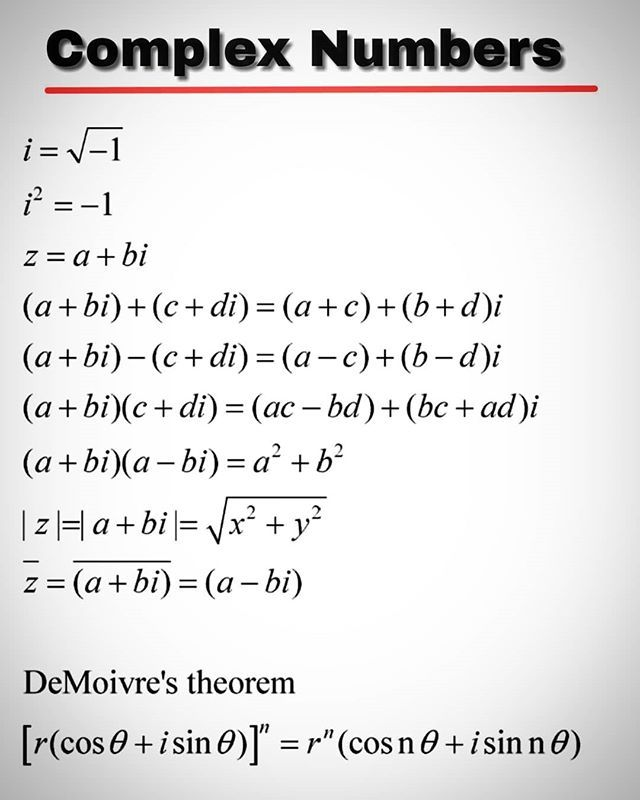
\includegraphics[width=0.5\textwidth]{complex_numbers.jpg}
\end{center}\end{center}
\end{frame}
\begin{frame}[fragile,label={sec:org19ffbb3}]{Aufgabe: Umschreiben des Spiels}
 \begin{itemize}
\item Schreiben Sie die Version des Spiels von der letzten Einheit
(Speichern von Monstern in einem {\color{solarizedYellow}\texttt{vector}}) so um, dass {\color{solarizedYellow}\texttt{Figure}}
keine Struktur sondern eine Klasse ist und wandeln sie alle nötigen
Funktionen in Member Functions um.
\item Überlegen Sie: Welche Variablen sollten {\color{solarizedYellow}\texttt{private}}, welche {\color{solarizedYellow}\texttt{public}}
sein?
\item Können Sie mehrere Konstruktoren sinnvoll einsetzen?
\end{itemize}
\begin{center}\begin{center}
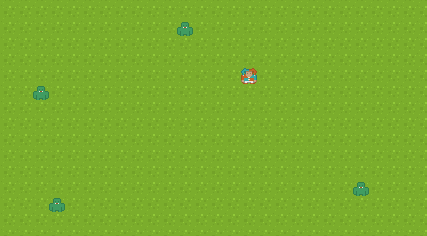
\includegraphics[width=0.5\textwidth]{screenshot-20200406-225138.png}
\end{center}\end{center}
\end{frame}
\end{document}